\newpage
\newsection{Serverless Framework}
\subsection{Description}
The Serverless Framework is a free and open-source web framework written using Node.js. Serverless is the first framework that was originally developed for building applications exclusively on AWS Lambda, a serverless computing platform provided by Amazon as a part of the Amazon Web Services.
\subsection{Serverless.yml}
One advantage of using this tool is the capability to deploy every time an entire serverless system based on cloud providers, in this case AWS. You can define a \emph{serverless.yml} configuration file which contains all the information about your service. You don't need to manually create the resources you need in a project, like database tables, queues, API endpoints and Lambda functions. You just have to write the code and then deploying your app.
\subsubsection{Serverless configuration for user management}
\begin{figure} [H]
This snippet of serverless configuration shows the name of your service, a list of plugins and the custom field. The \emph{dotenv} plugin is helpful if you have variables stored in a \emph{.env} file that you want loaded into your serverless yaml config. This will allow you to reference them inside your config and it will load them into your lambdas. Into custom field you have to declare the name of your variables.\\
The \emph{split-stack} plugin is useful when you reach the limit of 200 resources to deploy because it automatically split your resources using nested stacks.

\begin{lstlisting}[language=C]
	service: serverless-user-management
	plugins:
		- serverless-dotenv-plugin
		- serverless-plugin-split-stacks #to avoid the limit of 200 resources
	custom:
		splitStacks:
			perFunction: false
			perType: true
		dotenv: 
			include:
				- AUTH0_ADMIN_CLIENT_ID
				- AUTH0_ADMIN_CLIENT_PUBLIC_KEY
				- AUTH0_ADMIN_DOMAIN
				- AUTH0_USER_CLIENT_ID
				- AUTH0_USER_CLIENT_PUBLIC_KEY
				- AUTH0_USER_DOMAIN
\end{lstlisting}
	\caption{Service, plugins and custom - serverless.yml}\label{}
\end{figure}

\begin{figure} [H]
About your cloud provider: you can also define your IAM role authorization policies.
\begin{lstlisting}[language=C]
	provider:
		name: aws
		runtime: nodejs10.x
		region: eu-central-1
		stage: dev
		iamRoleStatements:
			- Effect: "Allow"
			Resource: "*"
			Action:
				- "dynamodb:*"
				- "sqs:*"
				- "lambda:*"
				- "cloudwatch:*"
				- "apigateway:*"
\end{lstlisting}
	\caption{Provider - serverless.yml}\label{}
\end{figure}

\begin{figure} [H]
You can define custom error responses from API Gateway, helpful to avoid CORS error.
\begin{lstlisting}[language=C]
	Failure500GatewayResponse:
		Type: 'AWS::ApiGateway::GatewayResponse'
		Properties:
			ResponseParameters:
				gatewayresponse.header.Access-Control-Allow-Origin: "'*'"
				gatewayresponse.header.Access-Control-Allow-Headers: "'*'"
			ResponseType: DEFAULT_5XX
			RestApiId:
				Ref: 'ApiGatewayRestApi'
\end{lstlisting}
	\caption{Custom gateway response - serverless.yml}\label{}
\end{figure}

\begin{figure} [H]
DynamoDB tables parameters: you have to define the name of the table, the name and the type of the key and the previsioned throughput.
\begin{lstlisting}
	UsersDynamoDBTable:
		Type: 'AWS::DynamoDB::Table'
		Properties:
			AttributeDefinitions:
				- AttributeName: userId
			AttributeType: S
			KeySchema:
				- AttributeName: userId
			KeyType: HASH
			ProvisionedThroughput:
				ReadCapacityUnits: 5
				WriteCapacityUnits: 5
			TableName: user
\end{lstlisting}
	\caption{DynamoDB table - serverless.yml}\label{}
\end{figure}
\begin{figure} [H]
 Lambda function and its handler: you can define which events trigger that lambda. In this case the event triggers the function when a new object arrives into the specified queue. 
\begin{lstlisting}
	commandCreateUser:
		handler: handler.commandCreateUser
		timeout: 10
		events:
			- sqs:
				arn: arn:aws:sqs:eu-central-1:582373673306:createUserQueue 
\end{lstlisting}
	\caption{Lambda triggered by SQS event - serverless.yml}\label{}
\end{figure}
 You can define an API gateway endpoint that triggers the corresponding function: you can also use a custom request template. If you want to protect the public endpoint you have to specify the authorizer function.
 \begin{lstlisting}
	readUser: 
		handler: handler.readUser
		events: 
			- http: 
			path: /readUser
			method: get
			authorizer: 
				arn: arn:aws:lambda:eu-central-1:582373673306:function:serverless-user-management-dev-admin_authorizer
				type: request
				resultTtlInSeconds: 0
			cors: true
			integration: lambda
			request:
				template:
					application/json: '{ "userId": "$input.params("userId")" }'
 \end{lstlisting}
\begin{figure} [H]
	\caption{Lambda triggered by GET endpoint - serverless.yml}\label{}
\end{figure}
\subsection{Project's root}
\begin{figure} [H]
	\centering
	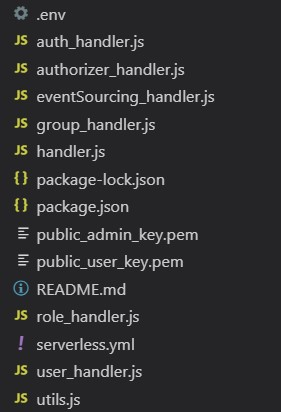
\includegraphics[scale=1.2]{../Img/root}
	\caption{Project's root}\label{}
\end{figure}
\begin{itemize}
	\item The main handler imports other handler's files: one per aggregate, one for authorizers and one to handle event sourcing functions. In this way the responsibilities are restricted to every type of aggregate;
	\item The \emph{utils.js} file contains a bunch of utilities functions; 
	\item The \emph{.env} file contains the environment variables loaded by the \emph{dotenv} plugin;
	\item The \emph{.pem} files contain the certificate provided by \emph{Auth0} to authenticate the client;
	\item The \emph{serverless.yml} contains the project's info and resources definition.
\end{itemize}
